\section{Introduction}
Equivariance describes how a learned representation responds to input transformations.
Let $f(x)$ denote the hidden representation extracted from the model for input $x$.
Let $G$ act on the inputs and let $\rho$ be an action of $G$ on the representation space.
The map $f$ is equivariant with respect to $\rho$ if $f(g\cdot x)=\rho(g)f(x)$ for every $g\in G$ and every input $x$.
In other words, the hidden representation of the transformed input equals the result of applying $\rho(g)$ to the original hidden representation.
The maps $\rho(g)$ compose according to the same group law as the input transformations by definition.
Prior work fits maps to paired representations \citep{lenc2015understanding} and studies when a transformation induces a well-defined map on the encoder's image \citep{sun2026transformationlaws}.
One approach is to learn the representation space and the group action jointly \citep{schmidt2025equivariance}.
We study how closely the existing hidden representations of a frozen language model can satisfy the equivariance relation for a prescribed group of input transformations.
On a fixed set of representations, we bound the minimum prediction error over exact orthogonal actions.
Under a common loss, we compare these bounds with the minima for independently chosen linear and orthogonal maps to separate the cost of orthogonality from the additional cost of enforcing the group law.
A low error under these constraints means that an exact action can closely predict the effects of the prescribed transformations on the representations.
The same representations may also support alternative actions that obey the same group laws but map states to different targets.
We therefore hold the representations fixed and compare the spectral budget of the prescribed action with those of the alternatives to assess whether the prescribed state correspondences receive stronger support.

We study two families of transformations on states named in the input.
In the weekday task, a one-day shift takes ``The current day is Monday.'' to ``The current day is Tuesday.''
Seven successive shifts return each day to itself, giving the cyclic group $C_7$.
In the square-corner task, a clockwise quarter turn takes NW to NE, while a reflection across the NW--SE diagonal fixes NW and SE and swaps NE with SW.
The rotations and reflections form the dihedral group $D_4$.
In both tasks, different state correspondences can obey the same group laws.
For example, swapping the positions of Tuesday and Wednesday in the weekday cycle changes Monday's successor to Wednesday while preserving the seven-step return.

Figure~\ref{fig:evaluation-targets} shows what changes in each evaluation.
For prediction, we fit maps on training templates and test them on held-out templates with the same state vocabulary.
The structural recovery and coordinate studies use separately constructed sets of templates and different prediction losses.
On each complete test bank in the coordinate study, we assess the cost of imposing exact action constraints while holding the representations, target pairs, and loss fixed.
We then compare the prescribed action with alternatives by changing the target pairs and computing the spectral budget of each action on the same bank.

% Keep the evaluation diagram near its first reference.
\begin{figure}[!htbp]
\centering
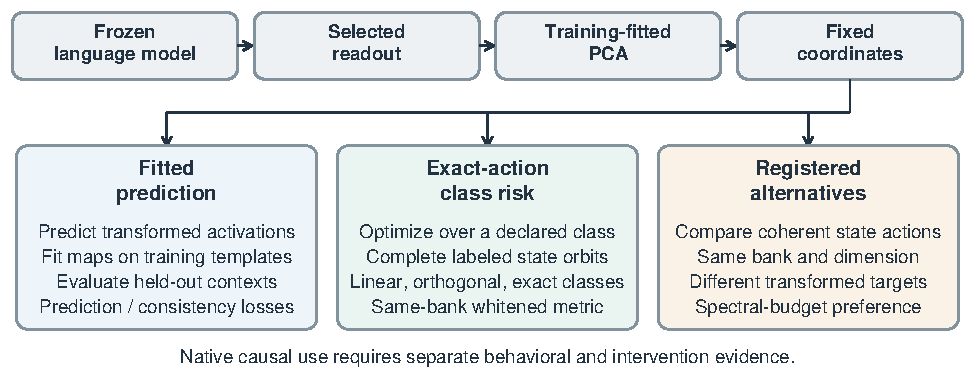
\includegraphics[width=\linewidth]{figures/evaluation_targets.pdf}
\caption{Three evaluation questions illustrated for a given bank of fixed representations. Fitted prediction scores learned maps on held-out contexts. Exact-action analysis bounds a class optimum in a declared metric. Registration comparisons change the coherent target action while keeping the source bank fixed. Each branch has its own evidence requirements.}
\label{fig:evaluation-targets}
\end{figure}

Our main theorem bounds the minimum prediction error $L^\star$ over exact orthogonal actions in a fixed real dimension $r$.
We compute a spectral budget from the orbit Gram matrix of the whitened representations and the group's action on its blocks.
The budget is the largest fraction of orbit energy that an invariant subspace of at most $r$ dimensions can capture.
The subspace must retain whole real irreducible components, so a two-dimensional rotation plane uses two dimensions of the budget.
In a constructed example, two systems have identical orbit-Gram eigenvalues and hence the same minimum error for independent linear maps.
Those eigenvalues belong to two one-dimensional components in one system and to a single two-dimensional rotation plane in the other.
With only one dimension available, the two systems have different minimum errors under exact orthogonal actions.
The spectral budget accounts for this difference and gives an upper bound on $L^\star$ that is at most twice the lower bound.

We evaluate both tasks in six frozen Llama and Qwen models.
In the structural recovery study, fitted linear maps reduce prediction error on held-out templates relative to the identity baseline.
In the coordinate study, the lower bounds on the additional cost of enforcing the group law beyond orthogonality vary widely across model and layer conditions.
In the 16-dimensional weekday analysis, a single condition accounts for 99.44\% of the sum of these lower bounds.
At the same dimension, the spectral budget of the prescribed action exceeds that of every alternative by more than the comparison tolerance in 7 of 24 weekday conditions and 16 of 24 square-corner conditions.
Reducing the retained dimension to eight changes both counts.

We also evaluate exact orthogonal actions constructed from training contexts as predictors on held-out contexts.
In every evaluated condition, the constructed action has higher prediction error than ordinary least squares fitted on the same training contexts.
A separate experiment evaluates two fitting objectives on newly authored context pairs containing the same state vocabulary.
We fit both predictors on the original training contexts, one to individual representations and the other to differences between paired representations of the same state.
We score both on their predictions of representation differences in the new pairs.
Relative to fitting individual representations, fitting differences lowers mean prediction error for weekdays and raises it for square corners.
Determining whether the model uses these transformations to compute its outputs would require behavioral and intervention evidence.

% Keep the introduction diagram before Related Work, without a fixed page number.
\FloatBarrier
